\documentclass[11pt]{report}
\usepackage{mathrsfs,graphicx}
\begin{document}

\noindent
George Weigt

\noindent
Homework \#2

\bigskip
\noindent
{\bf 1.} Write the differential equation for the following system.
$${C(s)\over R(s)}={
s^4+2s^3+5s^2+s+1
\over
s^6+7s^5+3s^4+2s^3+s^2+3
}$$

\bigskip
\noindent
See Ogata p. 55.
We have $n=\mathop{\rm deg} R=6$ and $m=\mathop{\rm deg} C=4$ with
$n\ge m$ as required.
Hence
$$a_0,\ldots,a_n=1,7,3,2,0,3\qquad b_0,\ldots,b_m=1,2,5,1,1$$
and the differential equation is
$$
{d^6y\over dt^6}+
7{d^5y\over dt^5}+
3{d^4y\over dt^4}+
2{d^3y\over dt^3}+
{d^2y\over dt^2}+
3y=
{d^4x\over dt^4}+
2{d^3x\over dt^3}+
5{d^2x\over dt^2}+
{dx\over dy}+
x
$$

\newpage

\noindent
{\bf 2.} Find the transfer function for the following network.
\begin{center}
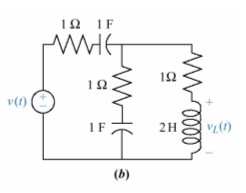
\includegraphics[scale=0.5]{images/210-1.png}
\end{center}

\bigskip
\noindent
The equation for the loop on the left:
$$1I_1(s)+{1\over s}I_1(s)+1I_1(s)+{1\over s}I_1(s)-1I_2(s)-{1\over s}I_2(s)=V(s)$$
The equation for the loop on the right:
$$1I_2(s)+2sI_2(s)+{1\over s}I_2(s)+1I_2(s)-1I_1(s)-{1\over s}I_1(s)=0$$
Hence
$$\left[\matrix{
2+2/s & -1-1/s\cr
-1-1/s & 2s+2+1/s\cr
}\right]
\left[\matrix{I_1(s) \cr I_2(s)}\right]
=\left[\matrix{V(s) \cr 0}\right]
$$
Solving for $I_2(s)$ we have
$$I_2(s)={(s^2+s)V(s)\over 4s^3+7s^2+4s+1}$$
The transfer function is
$${V_L(s)\over V(s)}={2sI_2(s)\over V(s)}=
{2s^3+2s^2\over 4s^3+7s^2+4s+1}$$

\newpage

\noindent
{\bf 3.} Find the transfer function for the following network.
\begin{center}
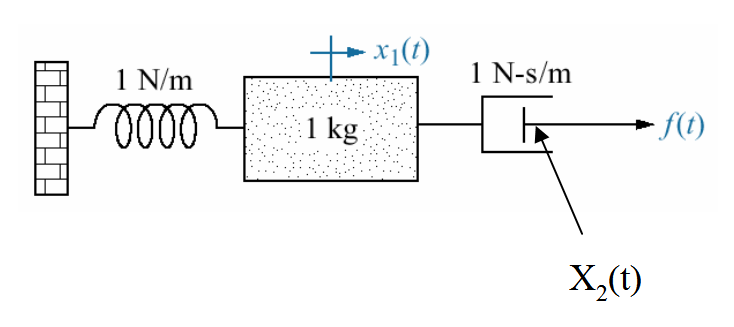
\includegraphics[scale=0.25]{images/210-2.png}
\end{center}

\bigskip
\noindent
The output we want to use is $x_1(t)$, not $x_2(t)$.
The $x_2(t)$ in the diagram is just a hint.
Hence we want to find
$$G(s)={X_1(s)\over F(s)}$$
There are four forces on the 1 kg mass.
\begin{verbatim}
                              --> x (t)
                              |    1
           2              ____|____
          s  X (s) <-----|         |<----- s X (s)
              1          |         |          1
                         |    M    |
                         |     1   |
             X (s) <-----|         |-----> s X (s)
              1          |_________|          2
\end{verbatim}
In the above diagram, $s^2X_1(s)$ is the force due to acceleration,
$X_1(s)$ is the force due to the spring and
$sX_1(s)$ and $sX_2(s)$ are the forces due to the damper.
(When $x_1(t)$ increases, the damper pushes back on $M_1$.
When $x_2(t)$ increases, the damper pulls on $M_1$.)
We have
$$(s^2+s+1)X_1(s)=sX_2(s)$$

\newpage

\noindent
To solve for $x_2(t)$ it is convenient to imagine a mass of zero attached
to the right side of the damper.
\begin{verbatim}
                              --> x (t)
                              |    2
                          ____|____
           s X (s) ----->|         |
              1          |         |
                         |    M    |-----> F(s)
                         |     2   |
           s X (s) <-----|         |
              2          |_________|
\end{verbatim}
(When $x_1(t)$ increases, the damper pushes on $M_2$.
When $x_2(t)$ increases, the damper pulls back on $M_2$.)
Since the mass is zero there is no force due to acceleration.
Hence
$$sX_2(s)=sX_1(s)+F(s)$$
By the two equations above we have
$$(s^2+s+1)X_1(s)=sX_1(s)+F(s)$$
Hence
$$X_1(s)={F(s)\over s^2+1}$$
Consequently the transfer function is
$$G(s)={X_1(s)\over F(s)}={1\over s^2+1}$$

\newpage

\noindent
{\bf 4.} Find the transfer function for the following network.
\begin{center}
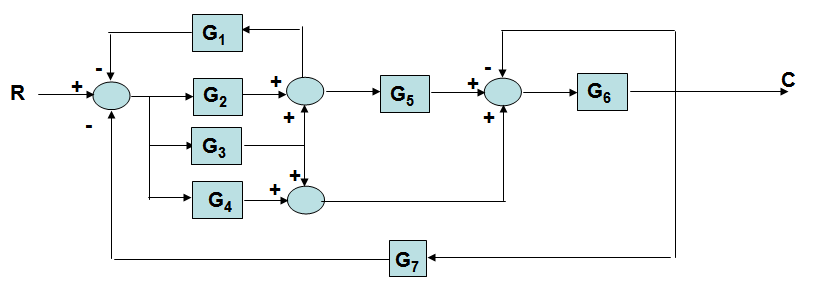
\includegraphics[scale=0.25]{images/210-3.png}
\end{center}

(Still working on the solution...)

\newpage

\noindent
{\bf 5.} Find the transfer function for the following network.
\begin{center}
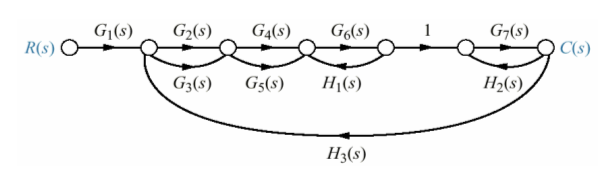
\includegraphics[scale=0.5]{images/210-4.png}
\end{center}

(Still working on the solution...)

\end{document}
